\documentclass[12pt, dvipsnames, a4paper]{article}
\usepackage{geometry}
\geometry{legalpaper, margin=0.5in}
\usepackage{xcolor}
\usepackage{lipsum,etoolbox}
\usepackage{xspace} 
\usepackage[normalem]{ulem}
\usepackage{vwcol}
\usepackage{cancel}
\usepackage{enumitem}
\usepackage{amsmath}
\usepackage{caption}
\usepackage{graphicx}
\usepackage{amsfonts}
\usepackage{float}
\usepackage{multicol}
\usepackage{hyperref}
\usepackage{listings}
\usepackage{textcomp}
\usepackage{lstautogobble}
\usepackage[parfill]{parskip}
\usepackage{tikz-qtree}
\usepackage{tikz}
\usepackage{hyperref}
\usetikzlibrary{decorations.pathreplacing}
\tikzset{every tree node/.style={minimum width=4cm,draw,circle},
         blank/.style={draw=none},
         edge from parent/.style=
         {draw,edge from parent path={(\tikzparentnode) -- (\tikzchildnode)}},
         level distance=1.5cm}

%% Genearl %%
\renewcommand{\thesection}{\arabic{section}}


%% For convenience %%
\newcommand{\code}[1]{\texttt{#1}}
\newcommand{\bcode}[1]{\texttt{\textbf{#1}}}
\newcommand{\balert}[1]{\textbf{\alert{#1}}}
\newcommand{\rarrow}{$\Rightarrow$}
\newcommand{\tab}[1][0.5cm]{\hspace*{#1}}
\newcommand{\deepemphasis}[1]{\underline{\textbf{\Large{#1}}}}
\newcommand{\bfemph}[1]{\textbf{\emph{#1}}}
\newcommand{\OR}[0]{\lvert \: \rvert}

%% Colours %%
\definecolor{mLightBrown}{HTML}{EB811B}
\definecolor{mLightGreen}{HTML}{14B03D}

%% Pseudocode %% 
\lstdefinelanguage{pseudo}
{
	keywords=[1]{
		let,
		class,
		new,
		loop,
		until,
		end,
		if,
		else,
		then,
		return,
		while,
		for,
		to,
		fun,
		break,
		and,
		true,
		false,
		or,
		do,
		max,
		min,
		elif,
	},
	keywordstyle=[1]\color{black}\bf,
	keywords=[2] {
		invariant,
		precond,
		postcond
	},
	keywordstyle=[2]\color{blue}\bf
}

\lstset{
	breaklines		=	true,
	language 		= 	pseudo,
	basicstyle		=	\ttfamily,
	mathescape		=	true,
	escapeinside	=	||,
	tabsize			=	2,
	numbers			=	left,
	commentstyle	=	\color{OliveGreen},
	stringstyle		=	\color{mLightBrown},
	upquote			=	true,
	morestring		=	[b]',
	moredelim		=	[l][\rmfamily\itshape]{@},
	comment			=	[l]{//},
	morecomment		=	[s]{/*}{*/},
	commentstyle=\color{Gray}\ttfamily,
	showstringspaces=	false,
	showtabs		=	false,
	autogobble
}

%% Other %%
\setcounter{secnumdepth}{5}
\setcounter{tocdepth}{5}

% \patchcmd{<cmd>}{<search>}{<replace>}{<success>}{<failure>}
\patchcmd{\abstract}{\titlepage}{\titlepage% Insert ToC-writing after starting a titlepage
  \addcontentsline{toc}{chapter}{Abstract}}{}{}
\setcounter{secnumdepth}{3}
\setcounter{tocdepth}{3}

% Keywords command
\providecommand{\keywords}[1]
{
  \small	
  \textbf{\textit{Keywords---}} #1
}


%**************************************************************************************************************%
%______________________________________________________________________________________________________________%
\begin{document}
\title{\textbf{EECS 4314 - Bit Theory\\Architecture Report}}
\date{\Large \today}
\author{
	\large \textbf{Amir Mohamad}\\ \small amohamad@my.yorku.ca\\\\
	\large \textbf{Arian Mohamad Hosaini}\\ \small mohama23@my.yorku.ca\\\\
	\large \textbf{Dante Laviolette}\\ \small dantelav@my.yorku.ca\\\\
	\large \textbf{Diego Santosuosso Salerno}\\ \small nicodemo@my.yorku.ca\\\\
	\large \textbf{Isaiah Linares}\\ \small isaiah88@my.yorku.ca\\\\
	\large \textbf{Joel Fagen}\\ \small joefagan@my.yorku.ca\\\\
	\large \textbf{Misato Shimizu}\\ \small misato1@my.yorku.ca\\\\
	\large \textbf{Muhammad Hassan}\\ \small furquanh@my.yorku.ca\\\\
	\large \textbf{Yi Qin}\\ \small aidenqin@my.yorku.ca\\\\
	\large \textbf{Zhilong Lin}\\ \small lzl1114@my.yorku.ca\\\\
	\large York University\\
}
\maketitle
\newpage
\hspace{0pt}
\vfill
\begin{abstract}
	Software architecture refers to the high-level view of a software system, including all software components, their respective relationships (connectors), and the principles and guidelines of their structural and behavioural design. It provides a broad and abstract view of the architectural design, and encompasses the key concepts and structures of the system. Each of these elements, or abstractions, collaborate and interact with each other and give rise to a collaborative environment that makes a system more than a simple conglomeration of individual parts. The arrangement of these architectural elements and their interactions are critical to the overall success of the system.

	In the context of FreeBSD, a Unix-based operating system, its conceptual architecture defines the fundamental design principles, architectural styles, components and connectors that make up such a powerful computing environment. Some of its components are the kernel, the system libraries and user applications.

	FreeBSD is based on the BSD model, which started its development in 1993 with one single goal in mind: to provide software that can be used for any purpose. A series of evolutionary upgrades have been made by the thousands of contributors, committers and core members of the project.

	The structure of the operating system is composed of 8 main interacting components, which are: the Kernel Facilities, the Security Features, Memory Management, Generic System Interfaces, File System, Terminal-handling, Inter-process communication, and Network communication.

	The data and control flows in the subsystems of FreeBSD are as follows: (1) initialization starts with the BIOS and is taken over by the operating system through various boot programs, eventually leading to the user process; (2) inter-process communication is managed by BSD sockets; and (3) file system management is handled by the Zettabyte File System, which is under the control of the operating system and communicates with devices through ISA drivers. Memory management is handled by the system's memory manager, which uses virtual memory and handles kernel memory allocation through various system calls.

	In FreeBSD, concurrency relates to SMPng Architecture, which includes mutexes, shared/exclusive locks, semaphores, and condition variables such as those found in many other systems.

	The two main use cases of FreeBSD are the Shell, which allows for system interaction, and the Networking environment, which has robust capabilities over several protocols, such as HTTP and FTP.

	The modular, efficient and highly configurable software architecture of FreeBSD makes it such a popular choice for various systems, servers, embedded environments and desktop applications.
	\\\\
	\keywords{keyword1, keyword2, keyword3}
\end{abstract}
\vfill
\hspace{0pt}
\newpage
\tableofcontents
\clearpage

\section{Introduction}
An Operating System is computer software that manages computer hardware. FreeBSD is an open-source operating system based on Unix and widely known for its speed, stability, reliability, performance and security. However, whereas other operating systems combine features from Unix systems, FreeBSD is based on its own BSD model.
The FreeBSD Project started its development in 1993 with the goal to provide software that can be used for any purpose with no strings attached. The idea is that the code will get the widest possible use and provide the most benefit. As a result, the software architecture of FreeBSD is designed to be modular, allowing users to easily add or remove features as needed. On the other hand, and similarly to other Unix-based operating systems, the core components of the architecture include (1) the kernel, (2) system libraries, and (3) user programs.
In an operating system, the kernel is responsible for managing system resources, such as memory and CPU time. FreeBSD uses a monolithic kernel design, meaning that all device drivers and system calls are integrated directly into it. This allows for efficient communication between the different components of the operating system, and therefore results in faster system performance. The highly configurable and modular kernel supports over 300 system calls, which provide the means for a user program to ask the operating system to perform tasks on their behalf. As a mechanism to support memory management and CPU scheduling, FreeBSD uses demand paging, which is a technique that only loads pages as they are needed, and is very common in virtual memory systems.
One of the key features of FreeBSD's software architecture is its use of a hierarchical file system organised in a tree-like structure. In this sense, the root directory is located at the top of the tree and all other directories and files branch off from it. This organisation makes it easy to navigate and manage the file system, and also allows for efficient use of disk space.
FreeBDS has over 33,000 ported libraries and applications for desktop, server, appliance and embedded environments, and they provide a wide range of functions to be utilised by user applications. Some of these libraries facilitate networking and database management, and others are just standard C libraries to communicate with user programs.
Thousands of user programs and applications have been written for FreeBDS. Since it’s based on 4.4BSD, an industry-standard version of Unix, it is easy to compile and run programs for all user needs, whether it’s internet services, networking, software development, net surfing, or any other user needs.
Overall, the conceptual software architecture of FreeBSD is designed to be modular, efficient and configurable, making it a very powerful, flexible and popular operating system for the execution of a wide range of user tasks.

\subsection{Overview}
\lipsum[1]
\clearpage
\section{Architecture}
\subsection{Evolution}
\subsubsection{Origins}
As you may or may not know, BSD stands for Berkeley Software Distribution. “The University of California at Berkeley obtained a copy of Unix from Bell Labs in 1974. Over the following four years, Bell Labs and Berkeley enjoyed a strong collaborative relationship which helped UNIX to flourish”(1). This collaboration branched out into different systems, the one of interest here being BSD. This system was shared around the world while also carrying the requirement of paying AT\&T for a license first. Due to the commercialization of Unix researchers at Bell Laboratories were no longer able to foster community research. Although community research still continued, just through a different avenue; the Berkeley Computer Research Group, which could further coordinate and produce Unix releases1).
CSRG was able to make big contributions to UNIX, the major one being implementation of ARPANet protocols (TCP/IP). This implementation has been used long after as the basis for TCP/IP implementation which shows its significance.
Although this was under the licensing fee of AT\&T (\$50000), this caused many to request for the networking code and utilities to be provided under free licensing terms. Which led to the Networking Release 1. Keith Bostic brought up the idea of another release with even more BSD code, which would take a huge workload to rewrite many lines of code. This pushed him to make a very innovative move which set the standard for open source software, he enrolled developers across the world to contribute to this release, and in return they would be commended with name for their work on the project. This work resulted in Networking Release 2.
After this release different groups of development split into different branches all prioritizing different things. One group “initially focused continued development exclusively on the Intel x86 platform” (1) as well as inexpensive CD-ROM distribution and ease of installation became the most widely used BSD, this is FreeBSD.

\subsubsection{Releases}
Being an open-source platform, FreeBSD develops as a result of contributions from both its users and its developers. Collaboration is critical to its evolution, which focuses on creating new features, optimizing performance, and introducing additional layers of protection. Developers and users must first identify new system requirements and develop solutions for them in order to start the evolution process. The best suggestions are then chosen for execution after being discussed and assessed by the community.

Significant releases over the years have advanced the development of the FreeBSD system. Some of the most significant releases that demonstrate the system's evolution through time are the topic of this study.
The release of FreeBSD 4.0 was a pivotal moment in the system's development. A new package management system was added to the FreeBSD operating system with this version, greatly simplifying the process for users to install and manage packages. Additionally, FreeBSD 4.0 provided significant performance improvements and improved support for modern hardware, making it a more efficient and dependable platform for both residential and commercial use.
FreeBSD 5.0, published in 2004, was the first stable release that represented the system's growth. With the introduction of this release, the system started adding support for advanced multiprocessors, thread support, and the sparc64 and ia64 platforms. The most important new features were support for hardware virtualization, a new security architecture, and support for more sophisticated file systems like ZFS. These features were among the numerous new features that were added. Additionally, by streamlining the network stack and enhancing the operating system's virtual memory capabilities, this new version enhanced operating system performance.
Another key release in the development of the system was FreeBSD 7.0. This update improved the system by enhancing data protection features. This edition also saw the introduction of the ZFS file system, which helped users manage and safeguard their data. It is now much simpler for users to run many virtual machines on a single host thanks to better support for multi-core CPUs and hardware virtualization.


FreeBSD 11.0 brought changes to the systems networked capabilities an further evolved the system into one that could cater to most of its users needs. This release brought major updates to the system network stack. This greatly increased the performance and scalability of the system. In addition VIMAGE virtual networking system was introduced and more improvements were made to ZFS support bringing further security enhancements to its users for data protection.
To summarize, the evolution of FreeBSD over the years has been shaped by a series of key releases that have brought new features, improved performance, and increased dependability to the operating system. With the help of these updates, FreeBSD has evolved from a simple Unix-like operating system into a strong platform that can accommodate a variety of uses and applications.


\subsection{Functionality \& Structure}
As we all know, filesystem is an important part of all kinds of operating systems, and it might be the part that users feel most familiar.  The main function of filesystem is to store, input and output the files.  Because of that, there are several parts of the FreeBSD need to interact with it for sure.  First of all, filesystem needs the basic system facilities to help control.  After that, memory management and filesystem can’t work without each other.  Then the network communication part needs the support of filesystem as well since we often need to upload files.  The last but not the least, the filesystem is connected with inter-process communication since there might have file changes happened from processes.
Terminal handling is another important part of operating system.  The order we make by terminals like keyboards and mouses needs to be handled first and then pass to computer.  As a result, it needs to interact with all other parts that controlled directly by users, including generic system interface, basic system facilities and inter-process communication.
Inter-process communication basically used to help coordinate different process.  Like what mentioned before, it getting order from terminal handling part and help kernel facilities, memory management, and filesystem.  At the same time, network communication can be considered as a kind of process, so that it needs to interact with inter-process communication.
Network communication is the part of FreeBSD that responsible for internet.  It’s reason why we can communicate with each other through internet.  This part get input from inter process communication, basic system facilities and filesystem.  After that, it post output to security part first to make sure the data received are harmless.

\subsection{Control \& Data Flow}
What is the control and data flow among parts?\par
Data flow is how data flows among system components during processes. Control flow is the order of executions among components. The explanations below show how both flows are structured in subsystems of FreeBSD.\par
\subsubsection{Initialization}
In the initialization process, Basic input/output system (BIOS) with read-only memory (ROM) will be the first program appears in the flow. Under the control of BIOS, the processer finds the address \code{0xfffffff0} which contains the how-to of POST routines for low-level initializations. Then, as the last POST routine, BIOS follows an instruction, called \code{INT 0x19}, to reach out the address \code{0x7c00} and find a boot0 program. At the point when a boot0 program executes, the control will be taken over by the FreeBSD operating system. After taking over its control, the system will jump to multiple addresses to go through other boot programs and BTX server (boot1, BTX server, and boot2), and eventually reach a loader, which boots the system’s kernel. After the kernel completes its boot process, the control would be taken over by the user process, \code{init}, and it begins user-level configurations so that users can login and access to a shell. In multi-user operation, \code{init} calls a get tty (\code{getty}) program to call \code{login} out, and in single-user operation, \code{init} will be return to a root shell instead.\par
\subsubsection{Inter-Process Communication}
The major component for IPC in FreeBSD is a descriptor file, called BSD sockets. For example, to obtain an object on a web page, the system recognizes the object, which is encoded as a file, and utilizes a HTTP protocol to obtain more information on the object. These processes can be completed in the system’s kernel. Then, BSD sockets take care of the process of utilizing Transmission Control Protocol (TCP) and Internet Protocol (IP) to obtain the object from a server.\par
\subsubsection{File System}
For the processes of communicating with devices, Zettabyte file system (ZFS) takes a significant role in the system. ZFS is a system that handles general file system jobs as well as the volume management jobs, and it is under the control of the operating system. By combining multiple devices into a pool, it generates a large file system. Based on this file system, data can be exchanged between a hardware device and programs. For programs to obtain data, stored in a device, an ISA driver controls the communication between them, and it copies the necessary data from the device memory into the main memory. Moreover, if data needs to be stored in a device, the driver takes the data address and sends it to the device. Then, the hardware’s Direct Memory Access (DMA) mechanism allows the device to access the data.\par
\subsubsection{Memory Manager}
We can find a lot of components that the system’s memory manager handles. One of the responsibilities is kernel memory allocation, which the system utilizes virtual memory (VM) to handle page tables with addresses. For instance, system calls such as \code{brk} can be made by library functions (e.g., \code{malloc}) to control the allocation volume of a process, and the system’s kernel in the OS reach out to the main memory if necessary. The whole process here can be completed by the kernel in the system.\par

\section{Concurrency}
Concurrency and parallelism in FreeBSD are primarily driven by the SMPng Architecture. The SMPng Architecture shares a lot of the same primitives as other architectures, such as mutexes, shared/exclusive locks, semaphores, and condition variables. The SMPng design was introduced in FreeBSD Version 5, to better accommodate multiprocessing systems and improve scalability.

\subsubsection{Read and Write Locks}

The SMPng Architecture supports both read locks and write locks. Multiple threads can safely read a portion of data at the same time without it becoming corrupted. However, once write operations are introduced, locks are required to protect data. One method used to circumvent this issue is by simply using an exclusive lock for writes and a shared lock for reads. Another method is less commonly used. It involves having multiple locks for a portion of data, with a read lock for only one of the locks and a write lock for all of them.

\subsubsection{Giant Lock vs Fine-Grained Locking}

Older versions of the FreeBSD system would use one Giant lock for all of the kernel, but in later versions the Giant lock was removed for various parts of the system such as the device drivers, UFS file system, and network stack. Overtime, the Giant lock has been replaced with smaller, fine-grained locks which improves parallel performance and scalability with multi-processor systems. Another reason the Giant lock was overhauled was because of Giant lock contention. This occurs most frequently during kernel-heavy workloads, such as networking or storage, resulting in more delays as the CPU waits for the lock to be unlocked.

\begin{figure}[!h]
	\begin{minipage}[c]{0.4\linewidth}
		\centering
		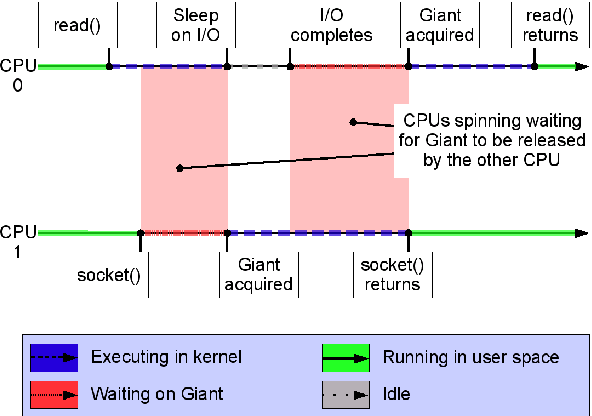
\includegraphics[width = 250pt]{assets/concurrency_diagrams/figureA.png}
		\caption{Giant Locking}
	\end{minipage}\hfill
	\begin{minipage}[c]{0.5\linewidth}
		\centering
		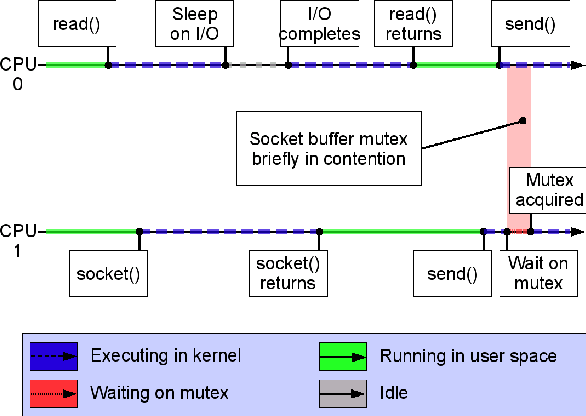
\includegraphics[width = 250pt]{assets/concurrency_diagrams/figureB.png}
		\caption{Fine-Grained Locking}
	\end{minipage}
	\caption{Comparison of different kinds of contention between Giant Lock and Fine-Grained Lock (Source: Watson) \cite{watson}}
\end{figure}

\subsubsection{Atomic operations}

The SMPng Architecture also supports atomic operations, i.e. a set of instructions that are protected together by a lock, without releasing the lock in between the execution of operations by a CPU. Atomic operations guarantee that after execution, all changes to the data made by a CPU are made visible at the same time to other CPUs. Atomic operations only allow one item to be read or written at a time.

\subsubsection{Interrupt Handling}

FreeBSD provides interrupt handlers with interrupt thread context, allowing them to block processes during execution, even with locks. The interrupt threads are often called heavyweight interrupt threads, because switching to them requires a full context switch. In order to mitigate latency, the kernel was made preemptive. Interrupt threads run at real-time kernel priority (ie the highest priority) and therefore, they should not run very long to avoid starvation. There are some interrupt handlers that don’t execute in a thread context, instead opting for primary interrupt context, but these handlers are only used in clock interrupts and serial I/O interrupts. In general, the CPU should be doing the highest priority work whenever possible.

\section{ The engineering process behind FreeBSD development }

The FreeBSD project is a unique collaborative venture that sees developers from around the world come together to contribute to and maintain an open-source operating system. It relies heavily on the dedication and commitment of its developers, requiring them to collaborate, compromise and work harmoniously to produce the best results. \cite{brooks} shows that increasing the number of participants increases the communication in the project exponentially. The creators of FreeBSD inherited the project model \cite{dev-model} approach to reduce the communications overhead. The project model is not meant to create impositions for participating developers, but its purpose is to act as a tool to facilitate interaction and coordination. This section will explore the implications of responsibilities among participating developers in the FreeBSD project and how these responsibilities can vary based on individual roles. 
\subsection{	Standards and guidelines}
The FreeBSD project requires developers to adhere to certain standards and guidelines for successful outcomes. To ensure that the entire team works together effectively, each developer must take ownership of their own tasks and be confident in their abilities. This means ensuring that any code they contribute complies with the coding style guide set out by the team, any tests written are accurate and complete, as well as making sure that any issues raised on GitHub or elsewhere regarding their work are addressed promptly. Moreover, communication between contributors is a must; this includes responding to queries in a timely manner and engaging positively in discussions relating to the project. Furthermore, it is important for developers involved in the project to stay up to date with changes made by other contributors so they can adjust their own work accordingly if necessary. This responsibility allows them to understand how each element has been incorporated into the wider system, as well as how it affects other parts of it. By taking responsibility for their individual roles within the FreeBSD project and adhering to established guidelines and standards, developers can help ensure its success.
\subsection{Collaboration tools}
There are various tools that enable developers to collaborate with one another and share their work on an online platform. These tools include issue tracking systems which allow developers to track tasks and defects in order to ensure progress towards a successful completion; access control systems which provide users with secure logins and permissions; versioning tools, so that different versions of code can be managed effectively; bug tracking systems, so any issues or bugs can be quickly identified and addressed; documentation repositories, where contributors can provide explanations for how certain features work; test suites enabling automated testing of code before it is released into production environments; and code review processes which help ensure quality standards are met. All these mechanisms combined mean that anyone looking to contribute something valuable has the resources they need at their fingertips while still being accountable for every line they write.

\subsection{Project Management Hierarchy}
FreeBSD project has a well-defined project management hierarchy. There is a Core Team that leads the project, a group of experienced developers who have commit rights to the source repo of FreeBSD, and finally there are contributors who despite not having commit right, help in advancement of the project. 
\subsubsection{Core Team}
The core team is a group of 9 individuals who are responsible for overseeing the overall direction of the project. These are experienced developers who have a long history of contributing to the project. 
\subsubsection{Project Lead and Committers}
Beneath the Core Team, we have the Project Leads. These are individuals who are responsible for specific areas of the project, such as the kernel, userland utilities, or documentation. They are the primary point of contact for questions and problems related to their area of expertise. Next up, we have the Committers. These are individuals who have been given the ability to make changes to the codebase. They review and merge contributions from others, and they work closely with the Project Leads to ensure that the code they commit is high quality and meets the standards set by the Core Team. 
\subsubsection{Contributors}
At the bottom of the hierarchy, we have the Contributors. These are individuals who have contributed to the project, such as submitting a bug report, writing documentation, or writing code. They play an important role in the development of the operating system, but they don't have the same level of decision-making authority as the other members of the hierarchy.
\begin{figure}[!htb]
	\advance\leftskip-0.5cm
	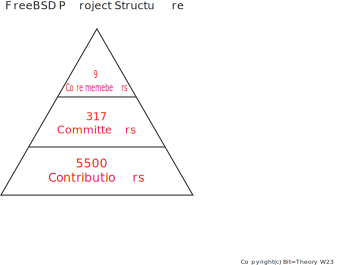
\includegraphics[width = 350pt]{assets/Project_Hierarchy/Project-Structure.pdf}
	\caption{Project Hierarchy of FreeBSD\cite{dev-model}}
\end{figure}



\clearpage
\section{Use cases}
\subsection{Shell}
The highest level use case of FreeBSD is using a shell to interact with the system.
Figure 1 shows how FreeBSD handles this use-case for a single user,
from starting up the system, to shutting it down. It's important to note that
this diagram showcases the flow in multi-user mode. If the system were in
single-user mode, \code{init} would return a root shell instead of going through the
\code{getty} and \code{login} process\cite{bootprocess}\cite{init}.

\begin{figure}[!htb]
	\advance\leftskip-0.5cm
	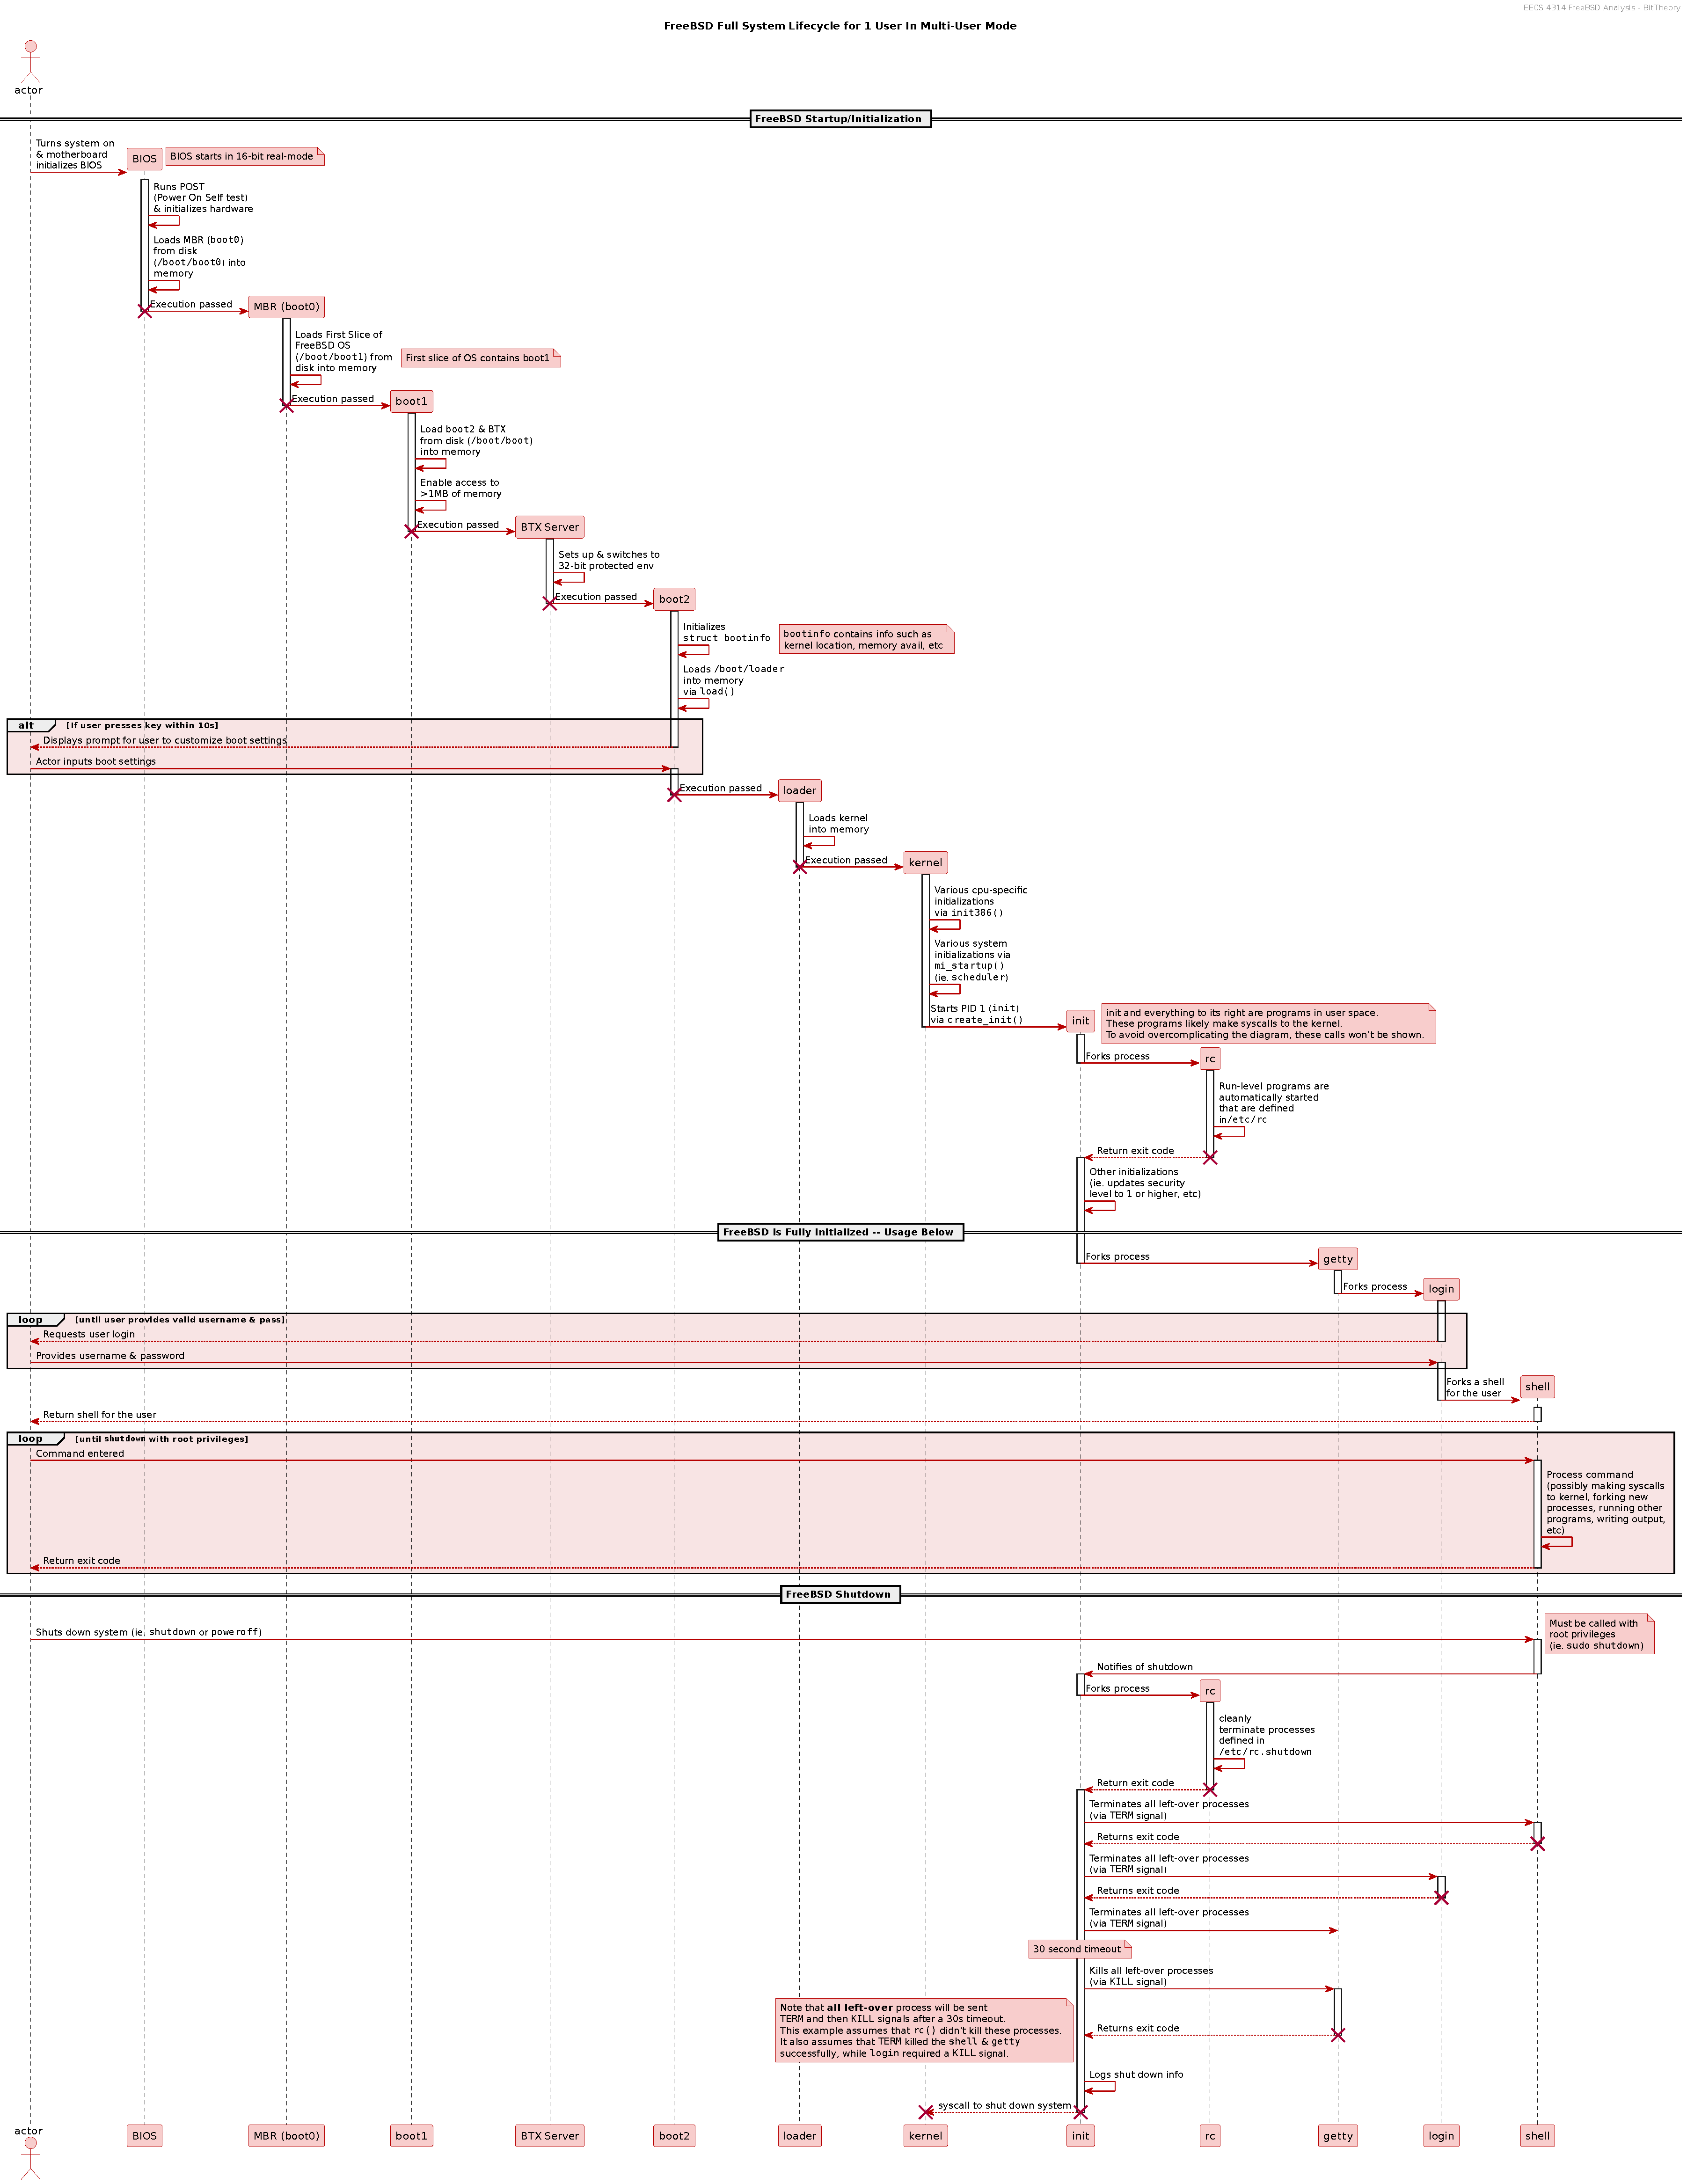
\includegraphics[width = 570pt]{assets/sequence_diagrams/system-flow.pdf}
	\caption{Sequence diagram of FreeBSD system-flow from startup to shutdown (In multi-user mode) \cite{bootprocess}\cite{init}\cite{getty}\cite{login}}
\end{figure}
\clearpage

\subsection{Networking}
One of the most important use cases of FreeBSD is the ability to network with other servers and systems. Because FreeBSD is
widely used as a server, as result it must have robust networking capabilities over several protocols such as \code{HTTP}, \code{FTP}, \code{NFS} and many more.
Figure 2 shows how FreeBSD handles a network request using the \code{HTTP} protocol using a browser. Please note that the default FreeBSD system
doesn't come with applications such as browsers or networking tools such as \code{curl} and they must be installed after initialization.

\begin{figure}[!htb]
	\advance\leftskip-0.5cm
	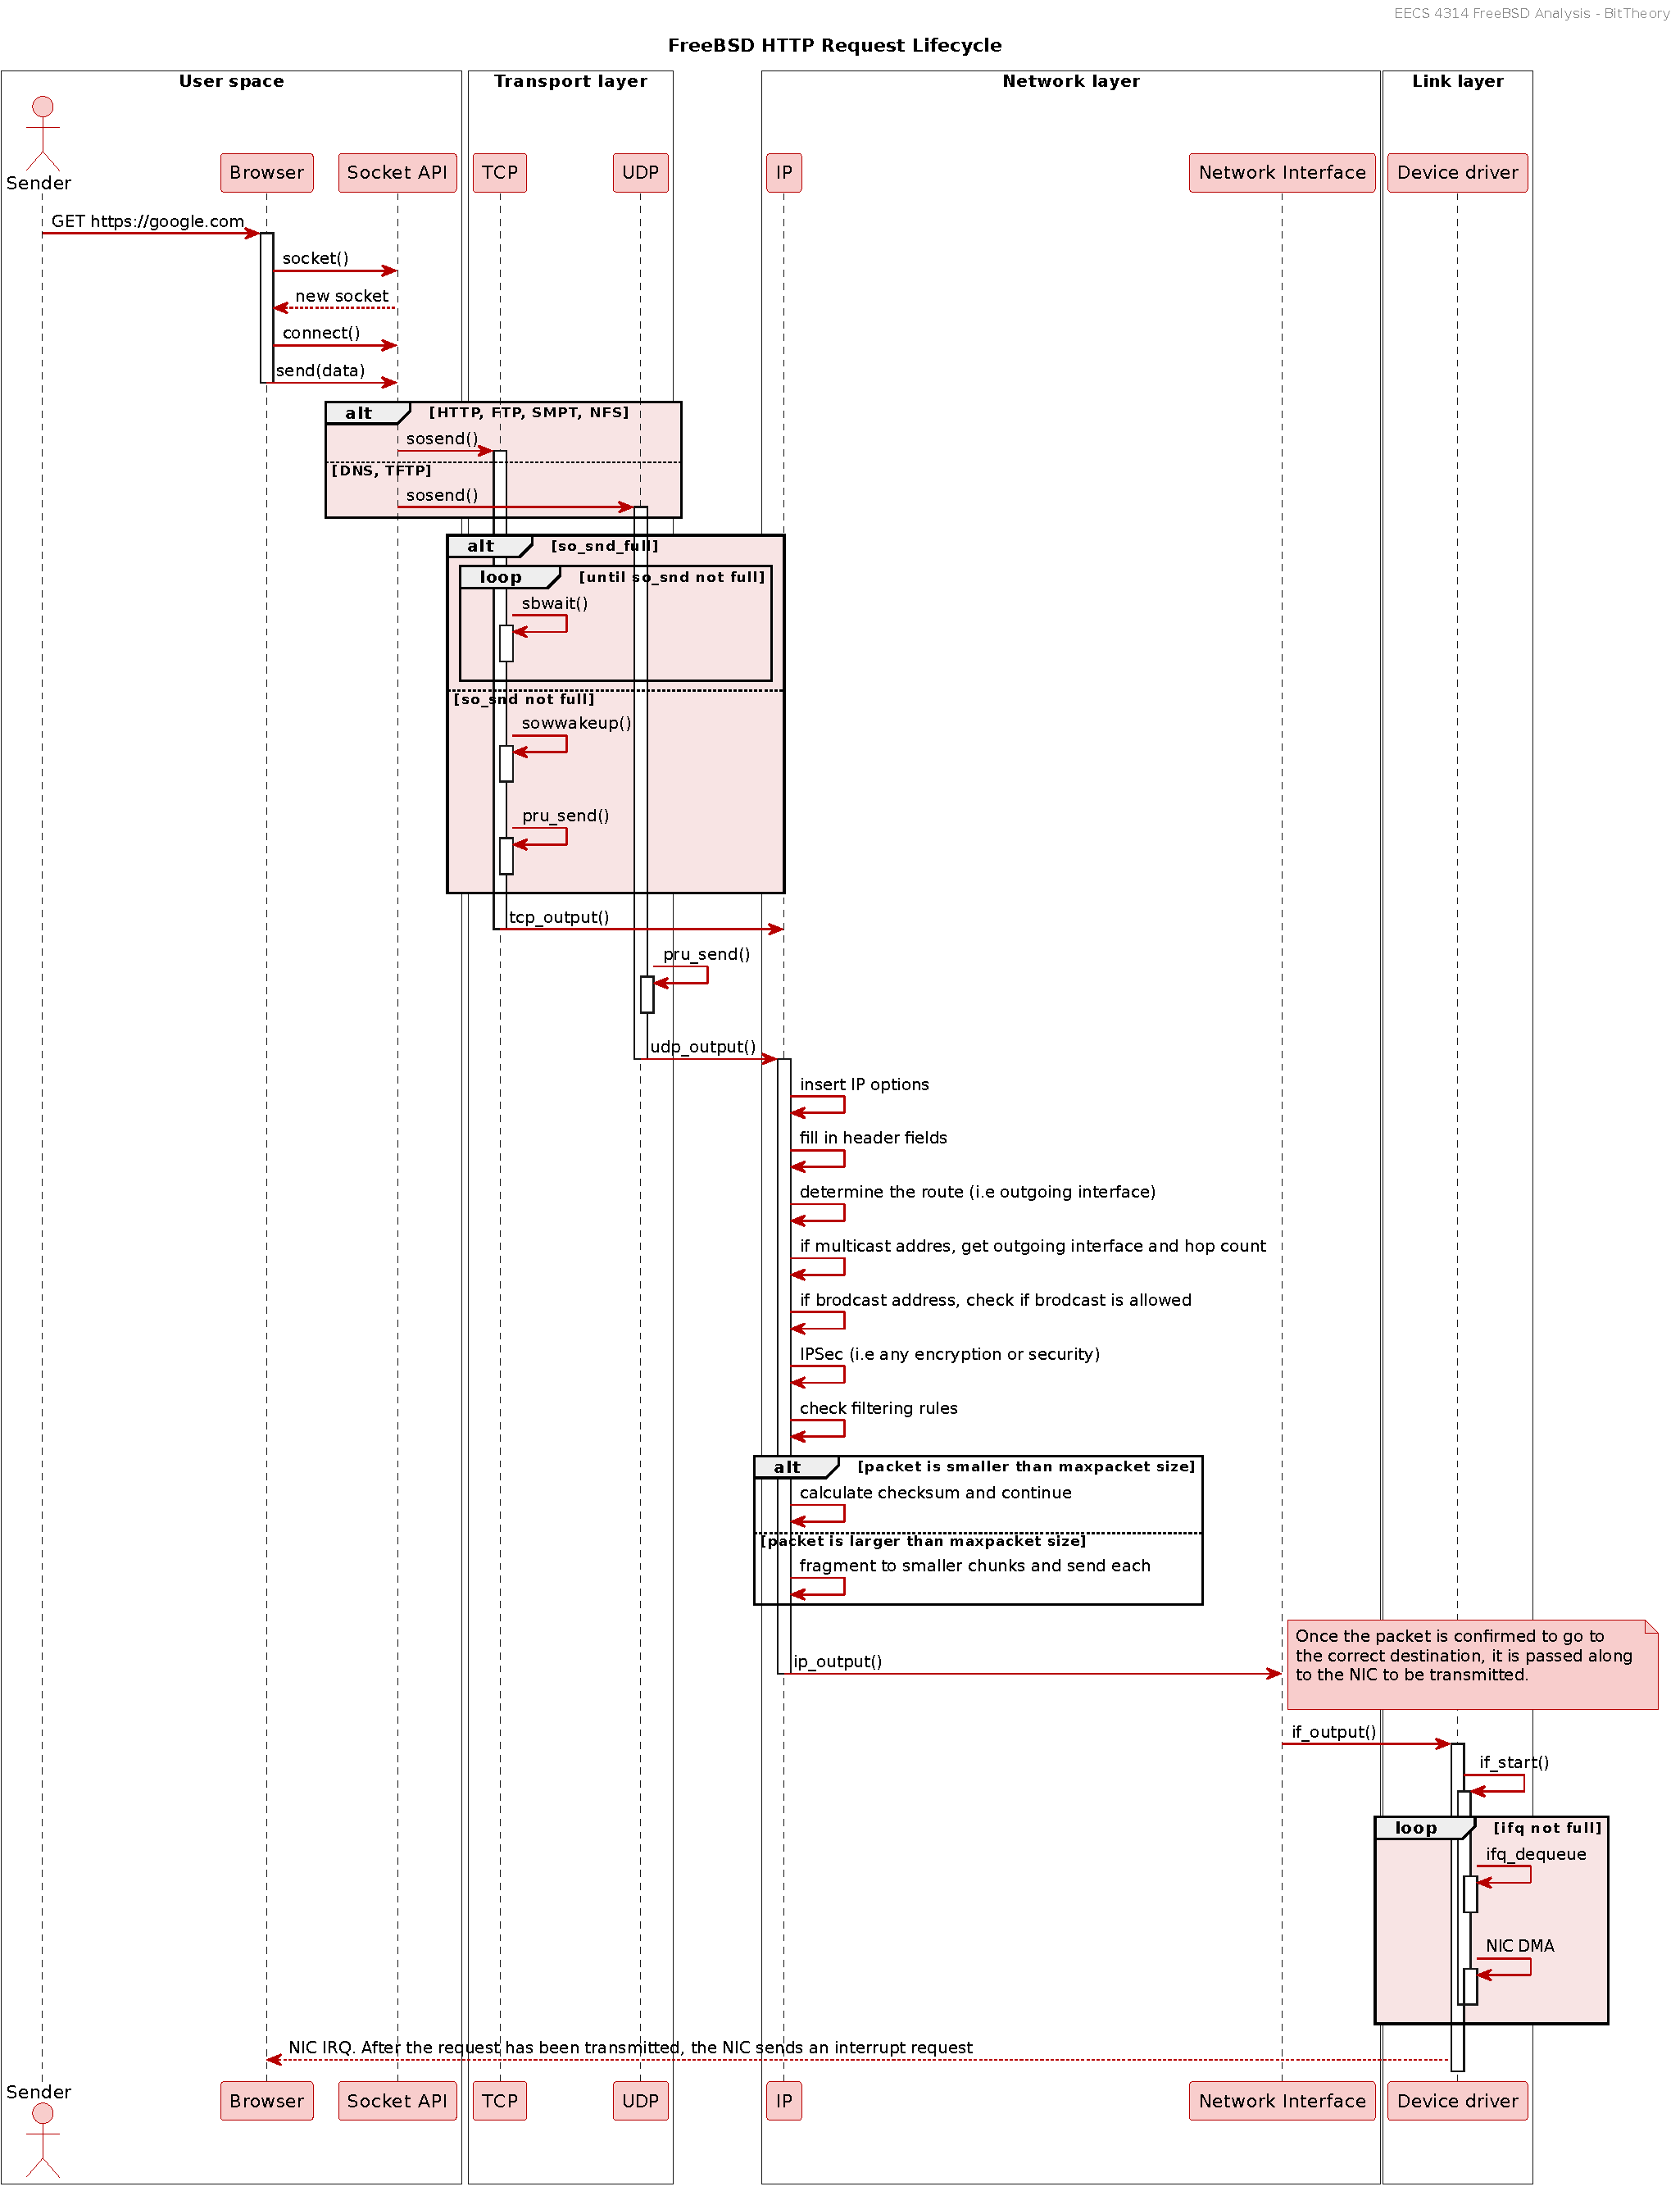
\includegraphics[width = 570pt]{assets/sequence_diagrams/network-send-flow.pdf}
	\caption{Sequence diagram of FreeBSD network-flow when a user makes an \code{HTTP} request}
\end{figure}
\clearpage

\section{External Interfaces}
\lipsum[1]

\section{Data Dictionary}
\lipsum[1]

\section{Naming Conventions}
\lipsum[1]

\section{Conclusion}
\lipsum[1]

\section{Lessons Learned}
\lipsum[1]

\begin{thebibliography}{00}
	\bibitem{brooks} Brooks, Frederick P. The Mythical Man-Month: Essays on Software Engineering. Anniversary Edition (2nd ed.). Addison-Wesley Pub Co, 1995. 
	\bibitem{smpng} "Chapter 8. SMPNG Design Document." FreeBSD Documentation Portal, https://docs.freebsd.org/en/books/arch-handbook/smp/.
	\bibitem{bootprocess} "Chapter 14. the Freebsd Booting Process." FreeBSD Documentation Portal, https://docs.freebsd.org/en/books/handbook/boot.
	\bibitem{dev-model} "FreeBSD Books." dev-model, https://docs.freebsd.org/en/books/dev-model/
	\bibitem{init} "FreeBSD Manual Pages." Init, https://man.freebsd.org/cgi/man.cgi?init.
	\bibitem{getty} "FreeBSD Manual Pages." Getty(8), https://man.freebsd.org/cgi/man.cgi?query=getty
	\bibitem{login} "FreeBSD Manual Pages." Login(1), https://man.freebsd.org/cgi/man.cgi?login\%281\%29.
	\bibitem{design} McKusick, Marshall Kirk, et al. The Design and Implementation of the Freebsd Operating System, 2nd Edition = FreeBSD Cao Zuo Xi Tong She Ji Yu Shi Xian, Di 2 Ban. Ren Min You Dian Chu Ban She, 2016.
	\bibitem{watson} Watson, R. "[PDF] Introduction to Multithreading and Multiprocessing in the Freebsd SMPNG Network Stack: Semantic Scholar." [PDF]  Introduction to Multithreading and Multiprocessing in the FreeBSD SMPng Network Stack | Semantic Scholar, 1 Jan. 1970, https://www.semanticscholar.org/paper/Introduction-to-Multithreading-and-Multiprocessing-Watson/088630aae6b4622e4175f58045cde69159d9eff5.
\end{thebibliography}
\end{document}
